\documentclass[12pt]{article}

% Margins
\usepackage[letterpaper, top=1in, bottom=1in, left=1in, right=1in]{geometry}

% For prettier tables
\usepackage{array}

% For pictures
\usepackage{graphicx}

% For units
\usepackage{siunitx}

\usepackage{float}

% For enumerates
\usepackage{enumitem}

% For code
\usepackage{courier}
\usepackage{listings}
\lstset{ mathescape }
\lstset{basicstyle=\ttfamily\footnotesize,breaklines=true}

% Clickable Table of Contents
\usepackage{color}   %May be necessary if you want to color links
\usepackage{hyperref}
\hypersetup{
	colorlinks=true, %set true if you want colored links
	linktoc=all,     %set to all if you want both sections and subsections linked
	linkcolor=black,  %choose some color if you want links to stand out
}

% For double spacing
\usepackage{setspace}

% Change Font
\usepackage[sfdefault]{roboto}  %% Option 'sfdefault' only if the base font of the document is to be sans serif
\usepackage[T1]{fontenc}

% For Header
\usepackage[english]{babel}
\usepackage[utf8]{inputenc}
\usepackage{fancyhdr}

% Make Header
\pagestyle{fancy}
\rhead{Andrews, Hickey}
\lhead{CS 467}

% Page numbers
\pagenumbering{arabic}

% Title
\title{Computers \textit{Attempting} to Kick Human Butt at Connect 4}
\author{Ben Andrews, Jimmy Hickey}

\begin{document}
	\maketitle
	\tableofcontents
	\clearpage

\doublespacing
\section{Introduction}
Connect 4 is a popular two player board game. It is an adversarial, turn-based game with rules that children can comprehend. The game is simple to understand, but requires decision making at each turn. This makes it a perfect subject for machine learning. WIth a small rule set, easily defined win conditions, and slow, turn based play a computer can be taught to play the game with some strategy.

\section{Problem Definition}
Our game board is a 7x6 matrix. When it is a player's turn, they choose a column to play a piece. They piece then falls to the lowest opening in that column; the players then alternate turn. This continues until one player connects 4 pieces in a row horizontally, vertically, or diagonally. 

We created methods to perform the following actions.

\singlespacing
\begin{enumerate}
\item Play the game on the computer.
\item Represent the game in a way a neural network could understand.
\item Generate our own data.
\item Train neural networks with our data.
\item Save these networks and reload them to play later.
\end{enumerate}
\doublespacing

\section{Project Goals}
Our initial intents were to teach both a supervised and unsupervised neural network to play the game. We then planned to pit them humans and each other. If trained on the same data, this would offer some insight into which method worked best for this type of problem.

However, our goals changed during the design phase. We decided to take a more data driven approach. We devised a system to generate data that could easily teach a supervised network to play the game.

Though we cut out our unsupervised network, we still wanted to compare techniques. Instead, we trained multiple supervised networks with various parameters. This allowed us to train networks to different efficacies. We can easily reuse our data to train more networks. 

We made networks that could play with noticeably different difficulties. These can play against humans, other AI strategies, random players, and each other. We are currently experieincing some difficulties that we believe arise from the data that we generated. Our next step would be to generate more, better data and continue training neural networks. We hope to have a network that is unequivocally better than a human.

\section{Model Formation}
\subsection{Choosing a Model}
Connect 4 is a solved game, meaning that given an board there is a mathematical best move. If perfect moves are played at each turn, the first player will always win. Though academically astounding, an AI that never loses is no fun to play against (trust us, we tried). Therefore, we decided to create a AI that is competitive, yet beatable. A minimax algorithm would do this well; however, this approach would takes a lot of time


 A supervised learning neural network generates moves in a $O (1)$ once it is trained, which is more usable for our purposes. Given this, we decided to create a neural network we could train to be competitive, but beatable, and that plays a move in an acceptable amount of time.

\subsection{Minimax}
Minimax is an adversarial search algorithm used in artificial intelligence. It is a common technique for game playing. 

It starts with the current state of the game board. From that it creates a tree. From the root, it creates a branch with its first possible move. It then creates another branch, again from the root, with its second possible move from the initial board state that it is given. It then expands the first created node via the same process. It continues down the tree until it is reaches a desired distance (this is it's depth or ply) or it reaches a leaf node. In our case, a leaf node represents a board that is full and cannot be played on any more.

Once the minimax tree is complete (either by it hitting the desired depth or finishing in all leaf nodes), it must be traversed. The last nodes created are evaluated and scored. This score is calculated based on the number of doubles (two pieces in a row), triples (three pieces in a row), a win (four pieces in a row), or an opponent win. The algorithm that we implemented assigned 1, 100, 100000, and -100000 points per respective pattern. The minimax algorithm models two players. The first tries to maximize the amount of points acheived. The second attempts to minimize the score. Depending on the depth of the search, this algorithm has the potential to generate a lot of nodes. Traversing can be very expensive; $\alpha - \beta$ pruning can help minimize this time expenditure.

The addition of the $\alpha - \beta$ pruning algorithm to the minimax algorithm can drastically reduce the search space of a problem. It prunes off branches that are assured not be chosen because of what has previously been seen in the tree. This reduces the amount of branches that need to be searched, improving the algorithm's speed. An example of this is shown in Figure 1.

Unfortunately, even with the addition of pruning, implementing a minimax algorithm to play against human players is not viable. A large branching factor is required for the tree to have any valuable insights; however this exponentially increases the search time, even with $\alpha - \beta$ pruning. In our experience, a 6-ply (6 depth) search took about 15 seconds per move, 7-ply took 500 seconds per move, and an 8-ply 6000+ seconds per move. This major disadvantage is what lead us to using a neural network. Though training it took a long time, it only needed to be trained once. Overhead was incurred only once and was not passed onto the user.


\begin{figure}[H]
\centering
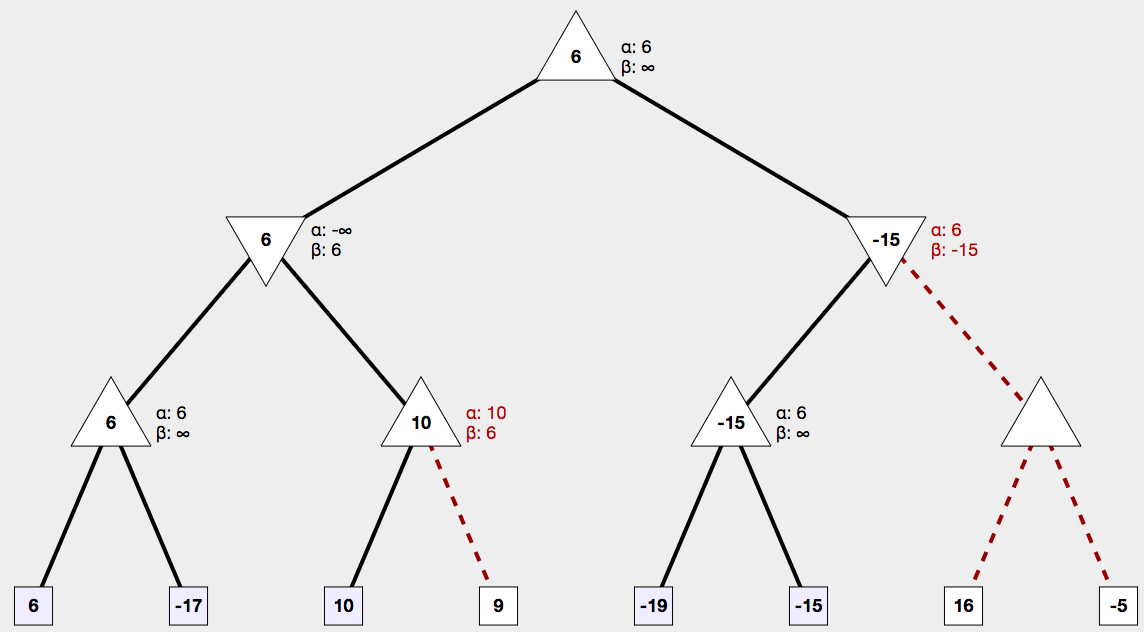
\includegraphics[scale=0.35]{img/alpha-beta.png}
\caption{Minimax with $\alpha - \beta$ pruning}
\end{figure}



\section{Implementation}
\subsection{Making the Game}
The game board is represented by a 7x6 matrix, made up of a list of lists in Python. Players play in columns; however, in our internal representation the rows and columns are flipped (see Figure 2). This allowed us to more easily store and retrieve the state of the board.  Empty slots are represented by a 0, Player 1's pieces are represented by a 1, and Player 2's pieces by a 2. When displaying the board to the user, we translated it back into a more recognizable and human friendly format (Figure 3). Empty slots are shown as a '-', player 1's pieces as an 'X', and player 2's piecess as an 'O'.

The player class is abstract. We implemented it a different way for each kind of player (human, random, minimax, and neural netwok). The only operation of a play is to play a piece in a selected column. After every play the board checks to see if there is a winner; to save computation time, the board only checks to see if the last move played created a winner scenario. This prevents checking the whole board for any winning permutation. If a winning scenario is found the game displays which player won and then ends the game.

\begin{figure}[H]
	\centering
	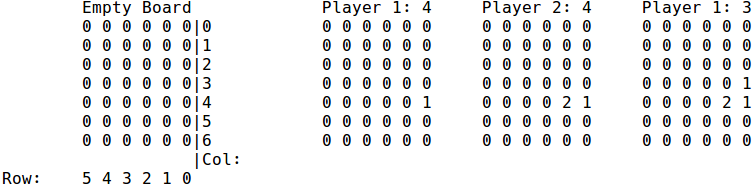
\includegraphics[scale=0.6]{img/rep_board.png}
	\caption{Internal Representation of the Board}
\end{figure}
\begin{figure}[H]
	\centering
	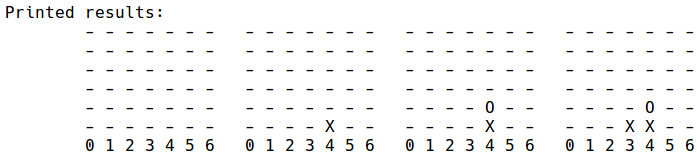
\includegraphics[scale=0.6]{img/print_board.png}
	\caption{Visual Representation of the Board}
\end{figure}


\subsection{Data Generation}
To train the supervised learning network we needed data. Each data point consists of a board state and the desired move. Our goal was to give the neural network as many different board states to learn from as possible. This would prepare a our network for a wide breadth of states that could occur in actual play. We determined that this was too big of a job to do by hand, so we implemented a minimax algorithm that we found on Github to help generate data. 

We made a new player object that used a minimax algorithm to make each move.
This \lstinline|make_move()| method converts our board representation to the one used by the minimax algorithm. It then calls the algorithm, passing the current state of the (translated) board and the depth which we would like to search. The algorithm then goes through creating a minimax tree and pruning. It then determines the best column to play in.

With this column information paired with the board state, we are ready to save a data point. We formatted these two parameters in a CSV. First, we flattened our board state into a one dimensional array. Again, this logical representation uses 0's to represent an empty space, 1's for player 1's pieces, and 2 for player 2's. We then saved the entries in this array and appened the desired column to the end. An example data point is shown in Figure 4.

\begin{figure}[H]
$$0, 0, 0, 0, 0, 1, 0, 0, 0, 0, 0, 1, 0, 0, 0, 0, 0, 1, 0, 0, 1, 2, 2, 2, 0, 0, 0, 0, 2, 1, 2, 1, 1, 1, 2, 2, 0, 0, 0, 0, 1, 2, 2$$
\caption{An Example Data Point with a Desired Column of 2.}
\end{figure}


\doublespacing

To automate the generation of this data, we needed something to play against the minimax algorithm. Since the minimax algorithm is guaranteed to make the best move given a board (and its depth), we could not use another minimax player. This would have result in the same game being played repeatedly. Instead, we created a random player that would play in a random column each move. This would also give us data for a vareity of game boards.

We decided on using a minimax player with depth 6; at around 15 seconds per move, it produced a good balance between move time and good move decisions. We decided that 1024 games would make as many different game states as we would need. Thus, we played the minimax against the random player 1024 times. Then, we switched their order, making the random player go first and the minimax second. If we did not do this, we would not have reliable data for player 2. All together, we generated 11,000 lines of data over 36 hours.


\subsection{Scikit-learn MLPClassifier}

We used the Scikit-learn Multiperceptron Classifier as our network. This gave us both the reliability of a production grade neural network along with the flexibility to adjust the parameters as we desired. Figure 5 shows an example of the general architecure of our neural network.

\begin{figure}[H]
\begin{lstlisting}[language=Python]
			MLPClassifier(activation="tanh",
				solver="sgd",
				hidden_layer_sizes=(10, 10),
				learning_rate_init=0.01,
				learning_rate='constant',
				max_iter=5000,
				batch_size=5000,
				shuffle=True,
				tol=0.00001)}
\end{lstlisting}
\caption{Example Neural Network}
\end{figure}

Let us explore each of these inputs individually.
\begin{itemize}
\item \textbf{\lstinline|activation:|} This determines the activation function that we used for our neurons. We went with the hyperbolic tangent instead of the sigmoid function because it teaches the network quicker (according to the slide shows).

\item \textbf{\lstinline|solver:|} This is the weight optimizer. We chose stochastic gradient descent (sgd) as it was the most similar to what we did in class.

\item \textbf{\lstinline|hidden\_layer\_sizes:|} This parameter is where we specified the dimensionality of our hidden layers. In the above example, we have 2 hidden layers, each with 10 nodes in them. This is the parameter that we changed to make neural networks of different competencies. Our most basic neural network had a single layer containing only 4 nodes. We then tried neural networks with 2 layers of 100 and 1000 nodes each.

\item \textbf{\lstinline|learning\_rate\_init:|} Our initial learning rate. This would be synonymous with the $\alpha$ that we went over in class.

\item \textbf{\lstinline|learning\_rate:|} This determines a characteristic about the learning rate itself. We experiments with both keeping it constant as well as setting it to ``adaptive." A constant learning rate does not change throughout the course of training. The adaptive learning rate changes the learning rate based on the performance on the network as it runs. If the error did not change over two consecutive epochs, the learning rate was divided by 5.

\item \textbf{\lstinline|max\_iter:|} The maximum number of epochs allowed.

\item \textbf{\lstinline|batch\_size:|} The amount of data used in each epoch. Going through all 11,000 lines of data each epoch would have taken even longer to train. We decided that 5000 randomly selected rows would add enough data to each epoch to learn while also supplying the network with a variety of data.

\item\textbf{\lstinline|shuffle:|} This randomized the order that the data was fed into the neural network. We wanted to ensure that the network would learn strictly on the board state rather than on the data surrounding it.

\item\textbf{\lstinline|tol:|} The tolerance for optimization. This determines the minimum amount that the error can change between epochs for the network to be considered trained.
\end{itemize}


\section{Computational Study}
\subsection{Performance of Minimax}
The minimax algorithm is very beatable even when at a depth that takes hours to return a move. We can attribute this blame across the computational speed of the minimax, and its heuristics. 

However, the minimax player always returns a valid move. It always makes a move to win or prevent the opponent from winning. Some strategy can be detected while playing against it. Further, minimax players that go down more plies consistently win against minimax players that are set to less plies. Overall, if we were to write a minimax player from the ground-up, we have determined a lot of improvements that we could make.



\subsection{Improvements to the Minimax Algorithm}
We used a na{\"i}ve minimax algorithm. Each time it looked at a board state in analyzed the whole board for doubles, triples, and wins. A more efficient approach would be to pass the board along with the current number of doubles and triples. This way, it would only have to calculate the new doubles, triples, and wins created by its moves. This is much more complicated algorithmically, but much more efficient computationally. 

Aditionally, we could add more increase the speed of the algorithm, allowing us to increase the depth without as much sacrifice. Currently, the whole system is written in Python, which is inherently slow. If we wrote Python extensions in C, or wrote the whole project in a compiled language, we would greatly enhance performance.

The minimax heuristics are also questionable. It calculates the score for each board state by counting doubles, triples, wins, and opponent wins. It does not, however, check and make sure that the double or triple it built could at any point become a winning play. For example, if the sequence of pieces hits a dead end on either side, from either hitting the edge of the board or the other player’s pieces, it will still get counted as points. This will improve the chances of making this move, though it gives no strategic advantage. Accounting for these edge cases would increase complexity and specificty of our minimax algorithm, but it would improve reliability

There are aditional changes that we could make to this heursitic. Since we cannot traverse very far down the tree due to time complexity, we cannot effectively predict an opponent's strategy. Instead of only tracking the minimax player's points (based on the doubles and triples), we would also track the opponents points. The overall value of a move would then depend on the net points it would afford the minimax player. Our algorithm would not only play what is best for it, but also try to minimize the opponent's gain in the process. This would add a layer of defensive play to our minimax algorithm. This is a major part of the strategy of the  game that our implementation currently does not support.

One final heuristic change we could make is adjusting the point values associated with each sequence of peices. Currently, having one triple is considered better than any amount of doubles. This heavily biases the algorithm to very aggressively go for triples. As previously examined, it will go for these moves even if they are not entirely strategically viable. Changing the point values correlated with doubles and triples would allow for more and different strategies.

If we were to completely recreate the minimax algorithm, there are some big overhauls that we could make to our current implementation to greatly improve reliabilty. We would implement a negamax algorithm. This is a modified minimax that plays the mathematically best move. It can have a much quicker response time than our current implementation. We started designing a player to use this modified algorithm, but did not complete it.

\subsection{Performance of the Neural Network}

We achieved our goal of creating a player that plays quickly. Our neural network responded with a move in under a second; however, there were a myriad of other problems with it.

 The neural network player always returned a column that exists, but sometimes returned a column that was already full. This move is invalid, and was rejected by the game board. This causes the game to call on the neural network player to play again. Since the board hasn't changed and the network had learned that that (full) column was the best move, it will try to play there again. This procedure repeates infinitely and must be interrupted externally.

Adittionally, the none of the neural network players played very well. We saw improvements as we increased the number of nodes, but even our best trained network could not play very strategically. Our better networks were able to beat our worse ones, however none of them could be the 6-ply minimax algorithm that produced the data that they were trained with. In fact, many of our networks lost to minimaxes as low as 2-ply. We can attribute this to poor training data.


\subsection{Improvements to the Neural Network}
We generated a lot of data for the neural network to train on. However, there are a lot of improvements that we could make to the data itself to improve future training.

As previously explained, we used a 6-ply minimax player. This depth was not very predictive, so we would like to increase to higher plys. This would give us data to train on from a better player. This fix would come with the speed and stability improvements previously outlined to the minimax algorithm.

A bigger problem arose from the design of our data generation. We played the 6-ply player against a random player. We thought that the randomness incurred from the random player would help to generate any unique board states. Unfortunately, it did not greatly impact our data.

The minimax player is programmed to make the best move for itself. In the beginning of the game, it will make the same moves every time. It will keep creating doubles or triples to sate its heuristic. To a human player, the minimaxes early strategy of making quick connections would be apparent; this is not the case for a random player. The random player would have to stop the minimax algorithm from winning within the first few move by sheer luck. Because of this, the minimax algorithm often won within the first few moves. Though we were able to generate a lot of data, much of it was redundant.

This issue could explain why our nerual network would play in invalid columns. It did not have sufficient data to have learned where to play when a column filled.

To remedy this issue, we have re-designed how we would generate data upon future iterations of our network. We would want to start the minimax player with a random board state every time. This would present it many different situations that are currently unexplored by our algorithm. We would implement this by playing two random players against each other. Doing this for a random amount of moves would allow us to generate new and unique board states. One of these players would then be swapped out with the minimax player, and our data taking would commence. 

With this improved  design, we would have a much wider variety of data to train the neural network on. It would be more general and able to play in many different scenarios.

\section{Conclusion}
We were successfully able to teach a neural network how to play Connect 4. We generated our own data by implementing other artificial intelligence game playing strategies. We learned a lot about machine learning in the process, and most important about what we did poorly. We have a lot of ideas on how to improve the current state of our application. 

\pagebreak
\section{Sources}
\singlespacing
\begin{enumerate}
	\item\href{http://scikit-learn.org/stable/}{Machine Learning Library for Neural Network}
	\item\href{https://github.com/erikackermann/Connect-Four}{Minimax Algorithm}
	\item\href{http://blog.gamesolver.org/}{Negamax Algorithm}
\end{enumerate}


\end{document}
